\section{Un constat critique}

Dans les communautés auxquelles j'ai contribuer (Mir) et plus largement dans ce que l'on appelle aujourd'hui "les sciences des données", j'ai pu observer des phénomènes récurrents qui sont, à mon sens, néfastes pour le bon accroissement de la connaissance.

Cette quinzaine d'années de tâtonnement et d'exploration de différentes approches algorithmiques en sciences des données m'ont amener a identifier deux problèmes récurrents qui se retrouvent pour la plupart des productions\marginnote{Y compris les miennes.} :
\begin{enumerate}
  \item l'absence de formalisme expérimental canonique et rigoureux qui permet d'orienter et de justifier son effort de recherche à peu de frais;
  \item l'ajustement aux données, que ce soit par des approches algorithmiques de types série de peignes, ou de méta paramétrisation qui amène le plus souvent à la production de données quantitatives coïncidentes et des conclusions qualitatives dont les bases expérimentales sont fragiles.
\end{enumerate}

empilage de données
approche inductive pure
discussion qualitative permettant de mettre en lumière certaines observations lors de la phase expérimentale

\marginnote{A titre critique, Bob Sturm poursuit depuis plusieurs années un travail "d'auscultation" des travaux effectués en mir et organise un séminaire intitulé "Horse" en référence à Clever Hans (edition 2014 \url{} et 2018 \url{}).}

Ce n'est bien entendu pas le cas de toutes les productions scientifiques et il n'est pas question d'accuser la communauté de "piper les dés" de manière ouverte. Ce sont des problèmes qui ont leurs sources dans la manière qu'un chercheur peut être reconnu dans le contexte actuel, problématique que j'aborderai en Section \ref{}.

On peut par exemple citer le travail remarquable de YLan Boureau dans le domaine hautement compétitif du traitement de l'image \cite{boureau2010learning}. Son étude, basée sur un protocole expérimental rigoureux étudie l'importance des différentes composants d'une chaîne de traitement, en particulier les étapes de codage et d'union. "While much research has been devoted to devising
the best possible coding module, our results show that with
linear classification, switching from average to max pooling
increases accuracy more than switching from hard quantization to sparse coding. These results could serve as guidelines for the design of future architectures."

Dans une première approche, on peut considérer qu'il est nécessaire de pouvoir comparer simplement et efficacement de nombreuses approches différentes dans un même formalisme expérimental.

Les deux questions qui se posent alors, auquelles je vais essayer de répondre à la lumière de ma participation à l'organisation de challenges

 mais est ce suffisant ?

Et est-ce finalement si important ?



Les challenges tels qu'ils sont pratiqués aujourd'hui sont une certes une avancées par rapport à l'approche 'mon problème, ma base de données, mon algorithme, ma métrique' qui peu avoir son intérêt dans des phases de défrichage thématique mais qui ne peuvent être raisonablement considérée une fois la problématique bien identifiée. Ils  ne sont en aucun cas satisfaisant pour une démarche expérimentale rigoureuse visant à répondre à une problématique scientifique. La principale raison étant la domination de l'approche "ingénieur" qui vise à répondre à une application pratique par un procédé plus ou moins automatisable et non d'améliorer les connaissances dans un domaine scientifique bien identifié\marginnote{La domination actuelle des méthodes ensembliste montrent pour la limite de la technique de mise en compétition qui est un élément neccéssaire à l'accroissement structuré de la connaissance mais oh combien non suffisant.}.


Pour répondre à la deuxième question, je prendrais l'exemple du mir où il est troublant de constater qu'une infime partie des publications font état de travaux effectués conjointement avec des musicologues. Or, qui connais mieux la matière que ceux qui la questionnent depuis des centaines d'années ? Certes, un dialogue est nécessaire car les deux communautés sont assez disjointes, autant en terme d'objectifs, que de vocabulaire et de temporalité\marginnote{Cette dernière étant, dans mon expérience, la plus difficile à mitiger lorsque q'un chercheur en ingéniérie cherche à collaborer avec des spécialistes de la perception ou de la cognition}. Il est à mon avis néanmoins critique pour l'avenir de toutes disciplines portant sur la science des données de ne pas oublier d'ou viennent ces données et que des savoirs vivants sont à notre disposition\marginnote{Pour combien de temps encore ?} qui peuvent nous permettre de poser des questions qui ont du sens et d'apporter des réponses qui auront encore un intérêt dans une dizaine d'année.

Au vue de toutes ces considérations, il m'est apparu comme important, au delà de mon implication dans l'interface sciences des données / perception, cognition, de revenir aux bases de la méthode scientifique pour étudier la faisabilité d'une recherche expérimentale qui soit plus rigoureuse.

\section{Méthodologie expérimentale en sciences des données (5)}

La définition d'une problématique scientifique pour étudier un sujet particulier est régie dans ses grandes lignes par la méthode scientifique. Issue de pionniers comme Francis bacon (cite novum organum), elle permet de faire une étape importante dans la qualité de notre appréhension du monde. L'apport des penseurs grecs et romains qui est parvenu jusqu'a nous porte essentiellement sur la nature et la définition de la vérité et finalement assez peu sur la bonne manière de l’obtenir.

On trouve par contre des éléments en Orient sur cette période, comme le rapporte ce dialogue attribué à Bouddha et un de ses disciples \marginnote{ Question : "Maître, comment savoir si quelque chose est vrai ou faux ? \\
Comment savoir ce qu'il faut croire ?" \\
Réponse :"Ne croyez pas en quelque chose simplement parce que
vous l'avez entendu. \\
Ne croyez pas aux traditions simplement parce que
elles se sont transmises depuis de nombreuses générations. \\
Ne croyez pas en quelque chose simplement parce que
tout le monde en parle. \\
Ne croyez pas en quelque chose simplement parce qu'on le trouve dans vos livres religieux. \\
Ne pas croire en quelque chose simplement en vous basant sur l'autorité de vos enseignants et de vos aînés. \\
Mais après une observation minutieuse et une analyse rigoureuse,
Quand vous trouvez que quelque chose est en accord avec la raison,
Et qui est propice au bien et au bénéfice de l'un et de tous,
Alors vous pouvez l'accepter et vivre en fonction. \\
Question : "Alors, Maître, cela signifie-t-il que nous ne devrions pas nécessairement croire ce que vous venez de répondre ?" \\
$K\bar{a}l\bar{a}ma Sutta$, Gautama Bouddha, 500 avJc}.

Cette traduction contient pour moi deux éléments importants : 1) son exposé simple du caractère fondamentalement mal posé de la quête de la vérité, 2) le caractère résolument pragmatique de sa résolution de la "tension sceptique". Face à l'absence de référentiel non discutable permettant de confirmer ou d'infirmer une thèse, même après tout le soin que l'on peut apporter à notre argumentation, et seulement si l'on peut démontrer son intérêt pour la communauté, on peut choisir de vivre avec si tel est notre souhait.

Reste donc que c'est l'observation minutieuse et l'analyse rigoureuse qui va régir cette prise de décision. Il est donc capital de disposer de protocoles solides pour fonder nos expériences. Il est pour cela important de prendre conscience que la manière dont on considère une pratique impacte nécessairement cette pratique. Cet aller et retour entre (i) pratique expérimentale et (ii) observation critique de cette pratique, constitue pour moi un fondement de la recherche moderne.

Cela s'incarne très bien dans la relation encadré / encadrant, par exemple dans le cas d'une thèse de doctorat. Le doctorant, poussé par la force de la jeunesse dispose d'un élan conséquent et d'un enthousiasme qui lui permet d'avancer malgré les nombreuses déconvenues qui sont le quotidien du chercheur. Sans vision globale de l'état des connaissances de la communauté et sans vision critique, de haut niveau, du travail effectué, il y a de fortes chances pour que les échecs soient les conclusions de ses efforts. C'est la fonction importante de l'encadrant que de mettre en perspective le travail effectué et de le placer judicieusement pour ajouter de la connaissance dans la communauté visée.

Néanmoins, il est à mon sens important que l'encadrant soit, sur d'autres projets l'encadré et qu'il garde un contact avec l'expérimentation, car sans cela, ses connaissances critiques resterons en arrière par rapport aux avancées de la pratique expérimentale\marginnote{C'est l'apanage des chercheurs confirmés que de pouvoir tenir ces deux rôles. Je trouve personnellement plus irche et plus efficace de mettre en place des structures d'encadrement informelles lorsque je suis en charge d'une investigation.}.

C'est bien connu, acquérir des connaissances sur une pratique peut se faire en pratiquant, si possible avec des personnes reconnues dans cette pratique. Il est sans doute vain de vouloir formaliser complètements ces savoirs, néanmoins, ne serais ce que peut être pour mieux les maîtriser et les transmettre, je me suis intéressé a ce problème pendant plusieurs années.

Je discuterai ici dans le cadre de la méthode scientifique moderne qui se définit comme un processus itératif et cyclique dans lequel nos connaissances sont continuellement révisées à l'aide d'un processus comprenant les composants suivants:
\begin{itemize}
  \item \textbf{Caractérisations}: observations, définitions et mesures
  \item \textbf{Hypothèses}: explications théoriques ou hypothèses d'observations
  \item \textbf{Prédictions} : raisonnement inductif et déductif à partir de l'hypothèse ou de la théorie
  \item \textbf{Expériences} : évaluation de la pertinence de chacun des éléments précédents
\end{itemize}

Il est difficile de produire des recommandations qui soient pertinente pour l'intégralité des étapes de la méthode scientifique. En effet, les trois premiers composants relèvent de l'état des connaissances dans la communauté et des "directions" thématiques prises par cette communauté. Chaque communauté scientifique doit réfléchir aux axes à privilégier, à l'allocation de ressources, etc. J'ai donc fait le choix de consacrer ma réflexion à la partie expérimentale de la méthode scientifique, les autres relevant plus d'un choix ou d'une inclinaison culturelle et politique\marginnote{Je n'exclu pas qu'il soit possible de produire des recommandations dans ces domaines, je pense simplement n'être pas assez expérimenté pour cela. La tentative serait pourtant d'intérêt, car de nombreuses personnes se retrouvent aujourd'hui à des postes décisionnaires sans nécessairement être assuré du recul et des connaissances suffisantes pour faire des choix éclairés, ou au moins explicitement motivés.}.

On dispose par contre pour la partie expérimentale d'un ensemble assez solide et fourni de méthodes et d'outils pour mener à bien cette étape. Ces connaissances nous proviennent essentiellement de la science du vivant (médecine et biologie) où les conclusions tirées des études effectuées ont, depuis longtemps, un impact important pour l'humanité. L'impact grandissant qu'auront les sciences des données dans les décennies qui viennent, nous incitent fortement à faire de même.

Même si la tâche de systématisation est moins ambitieuse pour le composant expérimental, il est bien entendu illusoire de pouvoir proposer à la communauté un environment d'expérimentation qui soit suffisament flexible pour permettre toutes les expériences utiles à la communauté. C'est néanmoins par ce biais que j'ai approché la question, en suivant le paradigme du \textsl{faire pour apprendre}. Durant plusieurs années j'ai donc développé l'outil \textsl{expLanes}\cite{explanes} que j'utilise avec bonheur pour mes besoins propres et ceux des personnes que j'encadrent. Cette plateforme expérimentale est basée sur une formalisation que je présenterai ici. Elle n'est probablement pas la plus élégante qui puisse être conçue, mais elle a l'immense avantage d'être rompue à la pratique, où les besoins en expressivité sont dominants.

image d p s
        o

En sciences des données comme dans d'autres sciences, le principe est d'étudier la sortie $s$ d'un processus $p$ en fonction de certaines données d'entrée $d$. On souhaite que $s$ soit la meilleure possible, en fonction d'un ensemble de critères mesurables, que l'on appelera ici des \textsl{observations} ($o$).

A des fins de reproducibilité, on supposera que $d$ est pérenne, \textit{i.e.} n'est pas modifié par $p$. $s$ et $o$ sont non volatils, \textit{i.e.} stockés sur disque. $p$ peut éventuellement être segmenté en plusieurs étapes de traitement, qui appliquées séquentiellement permettent de produire le même résultat ($s_2=s$ et $o_2=o$).

%image d p_1 s_1 p_2 s_2
%         o_1     o_2

\marginnote{Ce découpage peut se faire de manière analytique en considérant l'architecture algorithmique de $p$. Néanmoins, en pratique, ce découpage se fait de manière à optimiser le temps nécessaire à la production de $s$, voir Section \ref{} pour plus de détails.}

Le but de l'expérimentation est la confrontation de plusieurs alternatives concernant l'architecture de $p$. Nous nommerons \textsl{facteur}, un élément de design de $p$. Chacun de ces facteurs peut prendre plusieurs valeurs, que nous nommerons \textsl{modalités}. Nous nommerons également \textsl{condition expérimentale} l'ensemble des modalités permettant de paramétriser $p$. Pour déterminer la condition menant à la meilleure solution, l'exploration d'un plan expérimental est pour cela nécessaire. Dès que l'étude dépasse la trivialité, le coût d'exécution du plan complet (toutes les conditions expérimentales) devient prohibitif.

Il convient alors de judicieux choisir les conditions qui nous permettent de maximiser notre connaissances de l'influence des différents facteurs, et en particulier leurs interactions. En effet, supposer que tout les facteurs sont indépendants permet de linéariser l'exploration des conditions. Malheureusement, cette indépendance est rarement complètement vérifiée de manière expérimentale. Il convient alors de savoir juger ce degré d'interaction pour faire des choix éclairés. Une autre technique consiste à effectuer l'intégralité du plan expérimental mais en simplifiant le problème à résoudre, souvent en réduisant la taille de $d$ (nombres d'exemples ou dimensions). Cette approche est risquée car elle peut amener à des choix algorithemiques qui ne généralisent pas correctement si le jeu de données réduit n'est pas représentatif\marginnote{Condition difficile à vérifier en pratique.}.

La littérature en factorial design

exemple du designOfExperiment \marginnote{Voir la documentation de expLanes pour une mise en pratique de cet exemeple}

\subsection{Les étapes de l'expérimentation}

On considérera que l'expérimentation se compose de trois grandes étapes :
\begin{enumerate}
  \item \textbf{le design} : conception et implantation de $p$, mise en place du plan expérimental, paramétrisation de l'environnement d'execution, execution de tests de conformité
  \item \textbf{l'exécution} : exécution des conditions expérimentales choisies
  \item \textbf{la réduction} : conversion des observations générer par chaque paramétrisation
\end{enumerate}

Comme tout processus computationel, on peut mesurer l'accès aux ressources en terme de
\begin{itemize}
  \item calcul
  \item d'accès disque
\end{itemize}

local / distant

Chacune de ces étapes a ses besoins propres en terme de ressources. L'étape de design nécessite une capacité élevée d'interaction avec $p$. Il est souhaitable que $p$ puisse être exécuté localement, éventuellement avec une version réduite de $d$ pour assurer au maximum la qualité du développement de $p$ avant l'étape d'exécution.

L'étape d'exécution a pour but de réaliser la plus grande partie possible du plan expérimental demandé. L'interaction avec $p$ étant alors minimale, on peut déporter le calcul sur des machines distantes. Des possibilités d'analyse de l'exécution de cette étape sont cruciales pour optimiser le temps nécessaire a ce que cette étape.

L'étape d'exécution va produire un ensemble généralement grand d'observations qu'il sera necessaire de réduire pour produire un ensemble de données réduit permettant de nous informer sur le comportement de $p$ lorsqu'il est soumis à $d$. Même si le nombre d'observations est trop grand pour être apréhender directement pour un être humain, on supposera que le volume de données est suffisament faible pour pouvoir être manipuler localement.

La maîtrise du temps de calcul est un point crucial de toute planification expérimentale. Cela se fait par le contrôle du temps de calcul nécessaire pour une condition expérimentale donnée, ainsi que le contrôle du nombre de conditions expérimentales.

\section{Explanes}

Le projet expLanes est né d'une frustration grandissante de l'auteur au sujet 2) du coût de dévelopement nécessaire à la mise en place d'un protocole expérimental de qualité, 2) l'absence de canons dans ce domaine, et 3) du risque élevé d'erreurs durant l'implantation de ce protocole expérimental compromettant gravement la validité des résultats obtenus. La version actuelle, écrite pour l'environnement Matlab, a nécéssité trois de dévelopement et est maintenant stabilisée et utilisé en production.

Je présenterai cette plateforme expLanes à des fins d'illustration des concepts introduits precedemment et pour introduire des éléments nécessaire à la présentation des choix aritecturaux présentés ci après\marginnote{Pour des informations plus complètes, la documentation est dipsonible sur le site web dédié : \url{}.}.

\subsection{Architecture}

Le principe d'expLanes est de fournir un environnement complet permettant d'aisément mettre en place un protocole expérimental destiner à répondre à des questionnements relevants des sciences des données. En particulier, il allège et systématise certaines étapes incontournables de ce type de protocole de manière à accélérer le processus de production, réduire les risques d'erreurs, et faciliter la maintenance à long terme.

Son architecture logicielle se compose de quatre composants principaux :
\begin{enumerate}
  \item un module de commande
  \item un module de planification
  \item un module d'exécution
  \item un module de réduction
\end{enumerate}

Le module de commande permet de configurer l'environnement logiciel et matériel dans lequel sera exécuté la commande transmise par l'utilisateur. Toutes les commandes disponibles sont présentes à l'état statique dans un fichier de configuration qui est spécifique à chacun des utilisateurs. On peut, par l'intermédiaire de l'interpréteur modifier les valeurs de ces commandes ou en ajouter d'autres. Au sein du code de chaque étape de l'expérimentation, cette configuration est disponible via l'objet \texttt{config}.

Le module de planification permet de gérer le plan d'expérience. A partir d'un fichier de description de ce plan, il génère efficacement une version manipulable. L'utilisateur peut alors aisément sélectionner les conditions expérimentales qu'il souhaite exécuter ou visualiser grâce à un mécanisme de masquage. Supposons un plan expérimental composé de 4 facteurs de 4 modalités chacune, le masque suivant $${2 0 1}$$ spécifie que la commande associée doit s'appliquer aux conditions expérimentales avec la seconde modalité du premier facteur et la première modalité du troisième facteurs. Le plan expérimental correspondant comprend alors 16 conditions au lieu de  $256$ pour le plan complet.

exécution

séquencement des calculs
chargement et stockage des résultats
mesure de progression des calculs
récupération des conditions expérimentales générant des erreurs

réduction

récupération des observations correspondant aux conditions expérimentales spécifiées par le masque
visualisation de ces observations
production du rapport


\subsection{Eléments de contrôle utilisateur}

La plateforme expLanes permet grace a ces modules de proposer des interfaces normalisée pour toutes les étapes de l'expérimentation telles que :

\begin{enumerate}
  \item la conception : création ou modification des étapes de traitement
  \item la planification : définition des facteurs, de leurs modalités et des règles d'exclusion
  \item l'implantation : implantation de chaque étape de $p$ dans des fichiers dédiés
  \item la configuration : définition de l'environnement matériel où sera exécuter le
  \item l'exposition : choix des conditions expérimentales d'intérêt et définition du mode d'exposition utilisé
\end{enumerate}

Considérons que nous cherchons de manière empirique à obtenir des connaissances sur l'aire de base et le volume des formes géométriques tridimensionelles \marginnote{Le code de cet exemple est disponible à cette adresse \url{}}.

La création de l'expérimentation \textsl{geometricShape} se fait comme suit :
\mcode{expCreate('geometricShape');}
Nous pouyvons ensuite instnatier deux étapes de traitement, une qui se chargera du calcul de l'aire de la base:
\mcode{geometricShape('addStep', 'base');}
et une autre du volume :
\mcode{geometricShape('addStep', 'space');}
Nous nous intéressons à l'influence potentielle des différents attributs (forme, couleur, rayon, largeur, hauteur) sur l'aire de sa base et son volume. Nous considérons donc chacun de ces attributs comme des facteur expérimentaux avec des modalités données.

Les formes étudiées sont le cylindre, la pyramide et le cube :
\begin{lstlisting}
geometricShape('addFactor', ...
	{'shape', {'cylinder', 'pyramid', 'cube'}});
\end{lstlisting}
La couleur peut être bleu ou rouge, le rayon peut être de 2, 4, ou 6 mètres, la largeur de la pyramide et du cube peut être de 1, 2, et 3 mètres et la hauteur de 2, 4 ,et 6 mètres. On note ici une exclusion qui est courante dans tout plan expérimental de complexité raisonnable avec plusieurs approches mise en compétition, certains facteurs ne devront être explorés que pour une modalité d'un autre facteur.
\begin{lstlisting}
geometricShape('addFactor', {'color', {'blue', 'red'}});
geometricShape('addFactor', {'radius', '[2, 4, 6]', '', '1/1'});
geometricShape('addFactor', {'width', '1:3', '', '1/[2 3]'});
geometricShape('addFactor', {'height', '2:2:6', '2', '1/[1 2]'});
\end{lstlisting}
Cette série de commandes permet de spécifier le plan expérimental, disponible dans le fichier \mcode{geshFactors.txt} :
\begin{lstlisting}
Factors:
1    shape =  =  = {'cylinder', 'pyramid', 'cube'}
2    color =  =  = {'blue', 'red'}
3    radius =  = 1/1 = [2, 4, 6]
4    width =  = 1/[2 3] = 1:3
5    height = 2 = 1/[1 2] = 2:2:6
\end{lstlisting}
La ligne 5 peut se lire comme suit, le facteur "height" n'est pertinent que pour l'étape 2 et les modalités 1 et 2 du facteur 1.

Les deux étapes de traitement sont implantées comme suit. Chaque étape dispose de la même signature, la variable \textsl{config} expose la configuration de l'expérimentation, la variable \textsl{setting} la condition expérimentale courante, et la variable \textsl{data} expose les données produite par l'étape précédente ou les données d'entrée pour la première étape.

La première étape se charge du calcul de l'aire de la base de la forme géométrique. Pour les besoins de l'exemple, on suppose ici que $/pi$ n'est pas connu de manière précise, ce qui est simulé ici par l'ajout d'une certaine incertitude sur sa mesure.

\begin{lstlisting}
function [config, store, obs] = gesh1base(config, setting, data)

uncertainty = randn(1, 100);
switch setting.shape
    case 'cylinder'
        baseArea = (pi+uncertainty)*setting.radius^2;
    otherwise
        baseArea  = setting.width^2;
end
store.baseArea = baseArea;
obs.area = baseArea;
\end{lstlisting}

La seconde étape complète le calcul effectué par la première pour calculer le volume de la forme géométrique :
\begin{lstlisting}
function [config, store, obs] = gesh2space(config, setting, data)

switch setting.shape
    case 'cube'
       volume = data.baseArea*setting.width;
    case 'cylinder'
        volume = data.baseArea*setting.height;
    case 'pyramid'
        volume = data.baseArea*setting.height/3;
end

obs.baseArea = data.baseArea;
obs.volume = volume;
\end{lstlisting}

\begin{marginfigure}
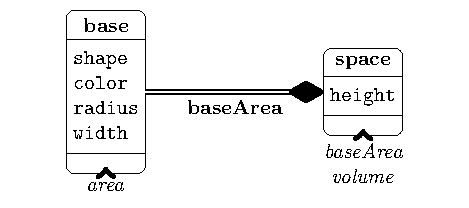
\includegraphics[width=1.2\textwidth]{figures/factors}
La commande \mcode{geometricShape('f')} génère un diagrame où les éléments principaux de l'expérimentation sont visibles (étapes de traitement, facteurs, données sauvegardées, observations).
\end{marginfigure}

Une fois l'implantation effectuée, le traitement est effectué avec la commande \mcode{'do'}. Par exemple, la commande \mcode{geometricShape('do', 1);} demande le calcul de l'étape 1 pour toutes les conditions expérimentales (qui sont au nombre de 18). Il est souvent nécessaire de ne pas effectuer le plan expérimental complet (étude spécifique, reprise sur erreur, ...), le mécanisme de masquage est alors utilisé. Par exemple, la commande \mcode{geometricShape('do', 0, 'mask', {[1 2] 0 1})} demande le calcul successif des deux étapes pour les cylindres de rayon 2 et toutes les pyramides.

Après le traitement des deux étapes, le répertoire dédié au stockage des données de calcul et d'observations contient :
\begin{tabular}{cc}

\end{tabular}

Ce n'est pas explicite dans cet exemple, mais les fichiers \mcode{_data} dédiés au stockage des données de calculs sont souvent de taille plus conséquente que les observations qui elle ont vocation à rester de taille raisonnable pour pouvoir être transférés des machines de calculs aux machines de visualisation et aisément analysées\marginnote{A noter également que pour toute expérimentation de taille raisonnable, les noms de fichiers peuvent être hashés pour ne pas dépasser les 250 caractères requis par la plupart des systèmes de gestions de fichiers.}.

A la fin du traitement, les observations de la dernière étape de traitement sont affichés :


La mise en forme précise de l'exposition de certaines observations est un élément nécessaire pour une expérimentation efficace. La plateforme expLanes dispose d'un grand nombre d'outils pour ce faire.

Par exemple, ce dernier affichage peut être ré-obtenu grâce à la commande suivante :
\begin{lstlisting}
geometricShape('display', 2, 'expose', '>', 'mask', {[1 2] 0 1});
\end{lstlisting}
La commande :
\begin{lstlisting}
geometricShape('display', 2, 'mask', {1 0 1},...
 'expose', {'t', 'obs', 2});
\end{lstlisting}
affiche les volumes (observations 2) de l'étape 2 pour chaque cylindre de rayon 2 triés par la première observation sélectionnée. La fonte rouge indique la plus haute valeur, et les valeurs bleues, celles qui ne sont pas statistiquement différentes, au sens d'un t-test par paires effectué entre les observations de la condition expérimentale et celle correspondant à la plus haute valeur.

\begin{margintable}
\caption{Visualisation sous forme de table \LaTeX.}
\begin{tabular}{llc}
color & height & volume \\
\hline
blue & 2 &  26.12$\pm$9.30 \\
blue & 4 & 52.23$\pm$18.60 \\
blue & 6 & \textbf{\textcolor{red}{78.35$\pm$27.90}} \\
red & 2 &  24.61$\pm$7.54 \\
red & 4 & 49.23$\pm$15.07 \\
red & 6 & \textbf{73.84$\pm$22.61} \\
\end{tabular}
\end{margintable}

\marginnote{Dans notre exemple, même si le cylindre bleu est plus volumineux que le rouge, cette différence n'étant pas significative, on peut en conclure expérimentalement que la couleur n'influe pas sur le volume. Il est aisé ici d'isoler la cause de variabilité due à l'incertitude artificiellement ajoutée à la valeur de $\pi$. Dans un cas réel, cela peut être beaucoup plus difficile.}

Une fois la phase d'analyse des résultats effectuée, nous pouvons alors communiquer les résultats grâce à la production de rapports d'expérimentation.


traduire l'exemple des figures geométriques


\marginnote{Cet exemple étant a visée pédagogique, le lecteur trouvera des exemples plus avancés sur le site de la plateforme expLanes. La plupart de mes productions scientifiques s'accompagnent d'une publication de l'expérimentation expLanes qui a permi de générer les données, comme ce travail de réplication \cite{lagrange2015}.}

\section{Réflexions sur la revue par les pairs en sciences des données}

Outil indispensable à la communauté scientifique, elle comporte néanmoins des risques pour le chercheur, c'est en effet à ce moment que les fruits de son travail sont exposés, à la critique, à l'utilisation abusive, ... C'est aussi une formidable opportunité pour voir son travail servir de base pour la recherche future.

On assiste, je trouve, actuellement à une "crise" de la revue par les pairs ou plus exactement une crise de la publication d'article, principalement à cause d'une normalisation d'une expression anglo saxonne "publish or perish" qui est, dans un nombre toujours plus grand de pays, devenue loi. Les nouveaux moyens numériques de diffusion facilitant cette inflation, le chercheur doit passer beaucoup de temps à écrire, mais aussi à relire, des articles dont le contenu s'allège en conséquence\marginnote{En considérant que le nombre de personnes dédiant leur carrière à la recherche scientifique est resté stable durant ces 50 dernières années, les estimations du nombres d'articles publiés (nbArticles.png) sont inquiétants.}. \marginnote{A ceci s'ajoute la position indéfendable des éditeurs qui par abus de position historique ne facilite pas l'évolution nécessaire. Comment expliquer au contribuable les sommes que l'on nous demande pour l'archivage sur internet de nos articles (environ 1500 euros pour un fichier d'une dizaine de Mo) ?}. Comme tout moment de crise, de nouvelles opportunités émergent également qui pourraient amener à une nouvelle implémentation de cette dernière étape de la méthode scientifique qui soit plus respectueuse du chercheur et plus effective pour la communauté. \marginnote{J'éviterai ici toutes questions concernant l'évaluation du chercheur, les produits de l'étape de la revue par les pairs n'étant pas à mon sens un outil approprié pour cet objectif.}

Dans une tradition issue de la physique expérimentale, la revue par les pairs se base sur une description aussi précise que possible du protocole expérimental et d'une discussion plus ou moins approfondie sur l'interprétation que font les auteurs sur les résultats obtenus. Ce format "article" est motivé par le fait que l'environnement expérimental est très couteux à mettre en place et difficilement transposable. Par accumulation d'expériences avec des protocoles expérimentaux d'une différence plus ou moins contrôlé, on arrive à s'approcher de ce que l'on peut penser être la vérité (figure sur le copper).

Dans le domaine de la sciences des données, on peut considérablement accélérer le processus de reproduction et d'extension, car il est plus aisé de mettre en place le paradigme de la recherche reproductible. En suivant la définition séminale de Donoho\marginnote{An article about computational science in a scientific publication is not the scholarship itself, it is merely an advertising of the scholarship. The actual scholarship is the complete software development environment and the complete set of instructions which generated the figures. \\—D. Donoho} et en l'étendant au cadre des sciences des données, on peut considérer qu'une contribution scientifique doit pour cela être composée:
\begin{enumerate}
  \item des données servant de base à l'expérimentation
  \item de l'implémentation qui, en fonction de ces données, produits les éléments quantitatifs discutés dans le compte rendu
  \item d'un article ou compte rendu d'expérience détaillant les hypothèses, le protocole expérimentale et les conclusions.
\end{enumerate}

Concernant la pérennité des données et de l'article, ces données numériques dites "statiques" ne posent pas de challenge particulier. Ce n'est malheureusement pas le cas du code informatique car il dépend d'une pérennité de l'interprétation de ce code sur les machines actuelles\marginnote{L'archivage et la maintenance du matériel qui a servi aux expérimentations n'est pas dans le cas général envisageable.}. Les difficultés de réplication pour cause d'obsolescence matérielle et logicielle sont endémiques de la recherche en sciences des données car cette activité se situe généralement dans des secteurs de pointe évoluant très rapidement\marginnote{Je citerai pour exemple l'évolution actuelle des bibliothèques de calcul sur unité de calcul graphique comme la bibliothèque cuda développée par nVidia. Indispensable pour tout traitement efficace d'architectures profondes, cette bibliothèque est propriétaire et les versions antérieures ne sont plus maintenues après quelques années.}.

Il reste que, bien souvent, une maintenance progressive du code par les auteurs au cours du temps permet de maintenir un certain niveau d'équivalence des résultats. Il est alors pour cela très utile de disposer d'un code qui soit bien structuré et facile à maintenir. Cette maintenance sera également grandement facilité par le choix judicieux des dépendances du code informatique publié. Si la phase d'expérimentation nous incite généralement à essayer de nombreuse approches, dont certaines très novatrices mais potentiellement instable et faiblement maintenues, il convient au moment de la publication de réfléchir à un bon équilibre entre apport scientifique et pérennité.

Garantir une reproducibilité complète pour un temps long de toutes ses productions est un défi probablement trop coûteux pour le chercheur. Il convient néanmoins de réfléchir en amont à cette problématique et d'allouer l'énergie nécessaire aux projets qui trouvent intérêt dans la communauté\marginnote{Les plateformes de développement collaboratif comme gitHub sont à ce titre particulièrement adaptées car elles permettent d'être informé de l'intérêt que porte la communauté aux travaux publiés et d'assister les collègues lors des tentatives de réplication.}.

Il est par contre aisé que les données expérimentales soient publiques et stockées de manière pérenne. Ceci doit être enforcé par la communauté\marginnote{Les plateformes de type archive ou zenodo sont de bons candidats.}. Même si l'implémentation particulière n'a pas vocation à être pérenne, il est bien évident que si les auteurs ont suivi un protocole expérimental canonique avec un effort de clarté et de concision dans l'implémentation, la réplication sera bien plus accessible. L'utilisation de cadres computationnels comme expLanes sont donc d'intérêt car ils permettent d'encourager de bonnes pratiques.
